\chapter{Avaliação da testabilidade de SMA $\mathcal{M}$oise$^{+}$ }

Em \cite{winikoff2014testability} um grafo de controle de fluxo foi utilizado para avaliar a testabilidade de um sistema BDI. A proposta deste trabalho é avaliar a testabilidade de um SMA utilizando o $\mathcal{M}$oise$^{+}$ como modelo de organização e empregando RP como ferramenta de descrição e análise.

Partindo como base o trabalho de \cite{winikoff2017bdi} o grafo de controle de fluxo apresentado na Figura \ref{fig:control_fluxo} será utilizado para apresentar a metodologia de transformação de controle de fluxo para RP. Na conversão de controle de fluxo para RP é considerado que cada nó será transformado em um lugar, e as ligações entre os nós, as arestas, são convertidas em transições que são conectados aos lugares por arcos. Logo o nó \textbf{S} que é o início do controle de fluxo é transformado no lugar \textbf{S}. Os lugares \textbf{S} e \textbf{A1} são conectados por dois arcos e pela transição \textbf{t0}, que é a transição disparada ao começar o programa.

O nó \textbf{a1}, está ligado a outros dois nós em uma estrutura de divisão de caminhos, onde uma das arestas significa a falha e liga com o nó \textbf{a2} e outra quando a ação tem sucesso acessando o nó \textit{Y} que representa que o programa foi realizado com sucesso. Para a transformação na RP é necessário incluir a transição \textbf{t1}, que é disparada quando a ação \textbf{a1} falha, unindo o lugar \textbf{A1} a \textbf{A2}, e também a transição \textbf{t6} unindo o lugar \textbf{A1} ao lugar \textbf{Y}, transição que é disparada quando a ação \textbf{a1}  é bem sucedida. Esta primeira etapa é apresentada na Figura \ref{fig:4-fluxo-rp0.png}.

\begin{figure}[ht]
    \centering
    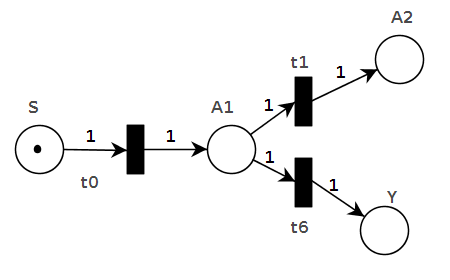
\includegraphics[scale=0.4]{imagens/4-fluxo-rp0.png}
    \caption{RP inicial.}
    \label{fig:4-fluxo-rp0.png}
\end{figure}

Como pode ser visto na Figura \ref{fig:cf_rp} a dinâmica da RP inicia pela indicação da \textit{ficha} no lugar \textbf{S}, quando a transição \textbf{t0} é disparada a ficha é movida para o lugar \textbf{A1}. Os arcos possuem o valor 1, significando que uma ficha já tem a capacidade de disparar aquela transição.

Em \textbf{A1} há uma estrutura de divisão entre diferentes sequências, onde e a transição \textbf{t6} é disparada quando é possível realizar a ação, indo assim para um lugar \textbf{Y} que corresponde à execução bem sucedida do programa, e finalmente para \textbf{E} que é o encerramento do programa. A transição \textbf{t1} é acionada quando o agente não consegue executar a ação \textbf{a1}, direcionando assim para o \textbf{A2}, esta ação pode ser bem sucedida, indo para a transição \textbf{t7}, ou falhar e ir para a transição \textbf{t2}, operando semelhante ao apresentado no \textit{lugar} \textbf{A1}.

\begin{figure}[ht]
    \centering
    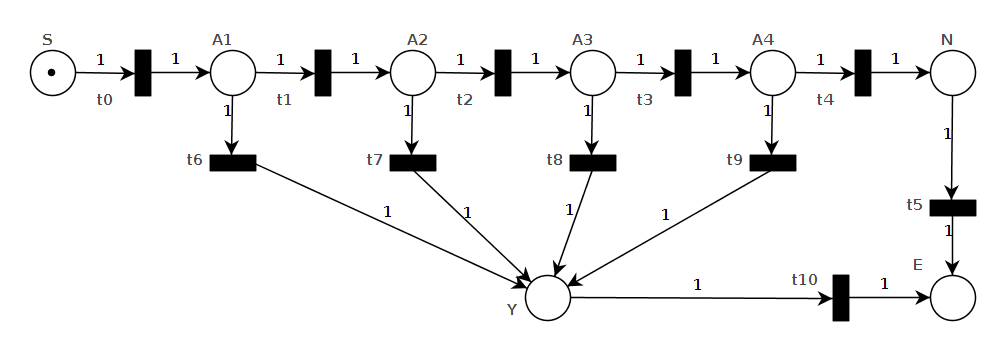
\includegraphics[scale=0.4]{imagens/4-fluxo-rp2.png}
    \caption{RP do grafo de controle de fluxo.}
    \label{fig:cf_rp}
\end{figure}

No método de \cite{winikoff2014testability,winikoff2017bdi} a avaliação de testabilidade é baseada na árvore de planos-metas, onde os objetivo tem como filhos os plano que são aplicáveis a ele, e cada instância do plano tem como filhos os sub-objetivos que ele publica, mas ainda apenas no nível de metas e ações. No contexto deste trabalho é necessário avaliar em múltiplos níveis que não estavam previsto em outros trabalhos, como missões, papéis e metas.



Em \cite{winikoff2014testability} a árvore de planos-metas é o pilar para seu trabalho, neste a avaliação da testabilidade no $\mathcal{M}$oise$^{+}$ será baseada no esquema social da especificação social, que é uma árvore de decomposição de metas. Para realizar a conversão do esquema social para RP é necessário convencionar a relação dos operadores apresentados na legenda da Figura \ref{fig:es_exemplo} e sua RP equivalente.

\begin{itemize}

\item Operador \textit{sequência}: representa uma cadeia de metas em sequência. A meta \textbf{G10} inicia a sequência, caso a transição \textbf{t1} for iniciada a ficha é retirada de G10 e é colocada em \textbf{G13}, permitindo assim o seguimento da cadeia. 

\item Operador \textit{escolha}: apenas uma das metas, \textbf{G8} ou \textbf{G9} podem ser adotadas, para isso o lugar \textbf{G7} recebe uma restrição, quando uma transição for disparada e a ficha for inserida no lugar \textbf{G7}, a outra transição será desabilitada, não permitindo assim que a outra meta seja realizada. 

\item Operador \textit{paralelismo}: significa que as metas \textbf{G5} e \textbf{G6} podem progredir paralelamente e de modo assíncrono, mas a transição \textbf{t1} só será disparada quando as duas metas estiverem concluídas.

\end{itemize}

\begin{figure}[ht]
\centering
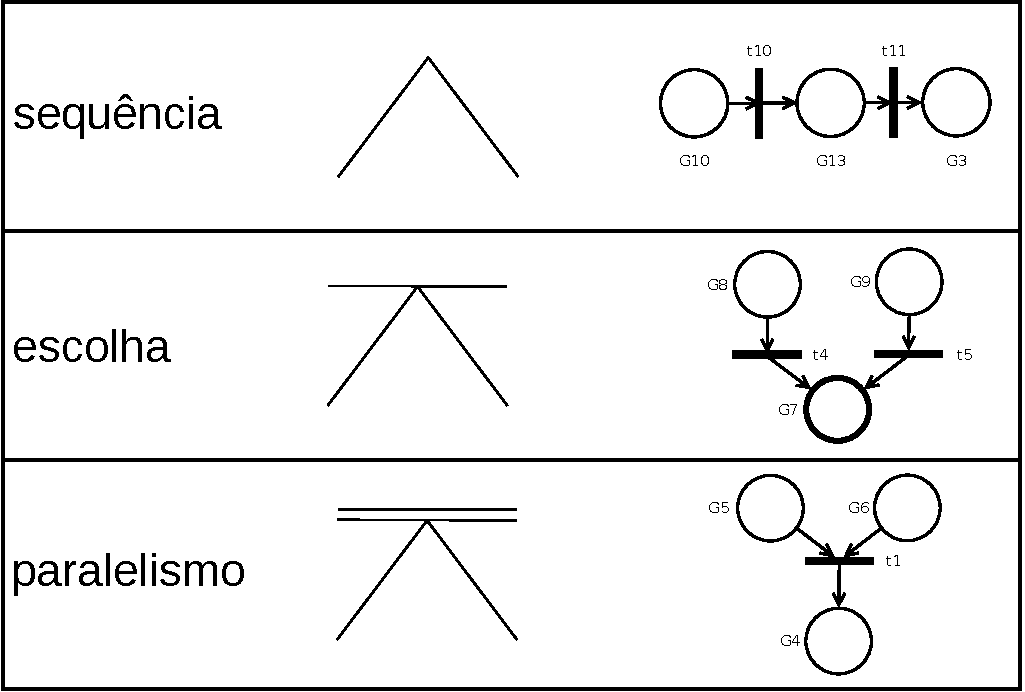
\includegraphics[scale=0.4]{imagens/4-relacao-moise-rp.pdf}
\caption{Relações dos operadores para Rede de Petri.}
\label{fig:moise_rp}
\end{figure}

Com a relação para a transformação dos operadores do esquema social para RP é possível criar a estrutura básica da rede, onde agora cada meta será um \textit{lugar}, semelhante ao que foi realizado na Figura \ref{fig:4estrutura_basica} onde cada ação foi transformada em um \textit{lugar}.  

Para atender ao nível organizacional é necessário utilizar recursos que não são disponíveis nas RP ordinárias, mas que podem ser modelados através de RP Coloridas. Na metodologia, as fichas coloridas são etiquetas empregadas na representação  dos papéis da organização. Os lugares se associam ao conjunto de cores das fichas, ou seja, sendo os lugares metas, então cada lugar terá a cor associada ao conjunto de papéis relacionados e de acordo com a especificação deôntica é possível correlacionar com a missão que representa aquele lugar.

Os arcos que ligam os lugares as transições recebem agora uma variável de cor (\textit{colset}) com valor pertencente ao papel, descrevendo qual cor está saindo do lugar e qual cor estará indo para o lugar de saída. Para o exemplo da Figura \ref{fig:es_exemplo} deve  ter um \textit{colset} que receberá os papéis, um \textit{colset} papéis, que será uma lista de papéis, e as variáveis que retratam as cores das transições. O código para declarar as cores na ferramenta CPN Tools encontra-se abaixo.

\begin{lstlisting}
colset Role = with candidato | secretario | membro | presidente;
colset ROLES = list Role;
var c, s, m, p: ROLES;
\end{lstlisting}

A linha 1 declara o \textit{colset} Role, que deverá conter todos os papéis presentes no modelo $\mathcal{M}$oise$^{+}$ utilizado.  A linha 2 é declarada ROLES que é uma lista de papéis (\textit{Role}), ela será a cor padrão dos lugares que em alguns casos recebem mais de uma ficha, ou então mais de um papel. E \textit{var} são as variáveis que representarão os papéis \textit{ROLES} nos arcos, limitando a maneira de como disparar as transições e quais cores devem ser colocadas nos lugares de saída.

Após inserir as declarações padrões para as novas cores é possível criar a RPC na ferramenta CPN Tools. Para o ES da Figura \ref{fig:es_exemplo} começando do canto esquerdo inferior da árvore. A modelagem da RPC pode ser dividida em 3 etapas.

\begin{enumerate}
\item Definição da estrutura da RPC: como primeiro conjunto de metas tem-se $g5$, $g6$ e $g4$ ligadas pelo operador paralelismo, logo utilizamos a Figura \ref{fig:moise_rp} para escolher a estrutura da RP para este conjunto de metas.
\item Inscrições da RPC:  como todas as metas possuem a mesma missão, todos os lugares receberão o mesmo conjunto de cor (ROLES), e sendo a missão $m1$  papel do candidato, os lugares iniciais recebem a ficha candidato. E as transições recebem c como inscrição representante dos candidatos.

\end{enumerate}

O resultado pode ser visto na Figura \ref{fig:RPC-1}. Na Figura \ref{fig:4-rp-exemolo1} é apresentada a RPC com as fichas de candidato nos lugares iniciais. É possível observar que a transição está ativada pela marcação verde que há nela, sendo assim todos os requisitos para disparar estão contemplados. Na Figura \ref{fig:4-rp-exemolo2} a transição foi disparada, ela está desativada e o lugar $g4$, lugar final, recebeu uma ficha, que é o valor de saída da transição mostrado pela variável $c$ do arco. Este exemplo mostra que, apesar de ter duas fichas candidato nos lugares iniciais, e apenas uma no lugar final, simboliza que o mesmo agente candidato se comprometeu com as metas $g5$ e $g6$.

\begin{figure}[ht]
  \centering
  \subfigure[RPC]{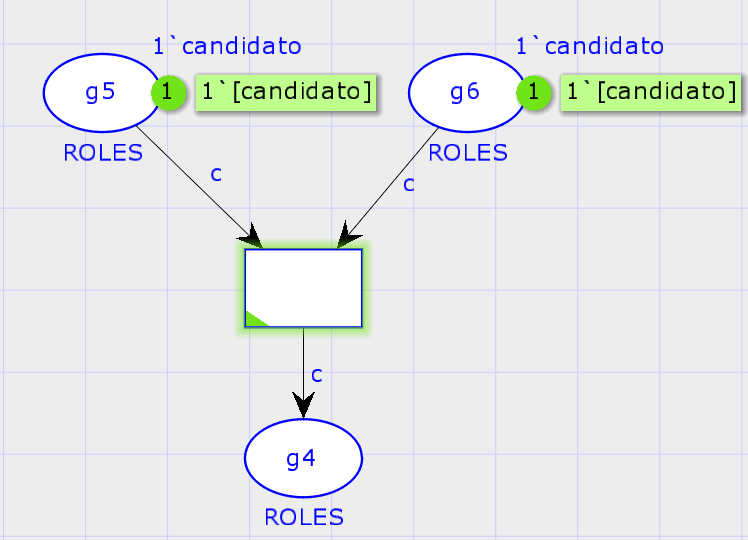
\includegraphics[width=0.47\textwidth]{imagens/4-rp-exemplo1.png}
  \label{fig:4-rp-exemolo1}}
  \subfigure[RPC com transição disparada]{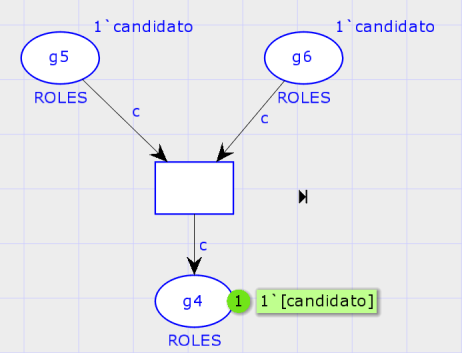
\includegraphics[width=0.45\textwidth]{imagens/4-rp-exemplo2.png}\label{fig:4-rp-exemolo2}}
  \caption{RPC das primeiras metas do ES}
  \label{fig:RPC-1}
\end{figure}

Na Figura \ref{fig:RPC-2} a RPC representa as metas $g11$, $g12$ e $g10$ da ES. Este conjunto de metas tem diferentes missões. A meta $g11$ em Verde-azulado (cerceta) é da missão $m3$ e recebeu a ficha "secretario", a meta $g12$ em oliva recebeu a ficha "membro" e faz parte da missão $m4$ e por último a meta $g10$, em vermelho escuro, faz parte da missão $m5$, representa a conclusão das metas $g11$ e $g12$, e é de responsabilidade do presidente. A opção de manter as fichas "secretario" e "membro" na missão $g10$ foi para simbolizar que um agente pode delegar as metas para outros papéis realizarem, e o responsável pela meta ter apenas que garantir que ela seja concluída.

\begin{figure}[ht]
  \centering
  \subfigure[RPC]{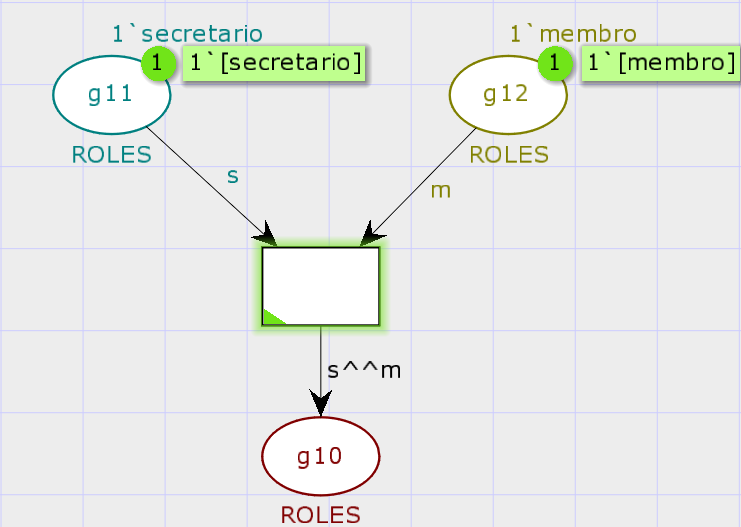
\includegraphics[width=0.47\textwidth]{imagens/4-rp-exemplo3.png}
  \label{fig:4-rp-exemolo3}}
  \subfigure[RPC com transição disparada]{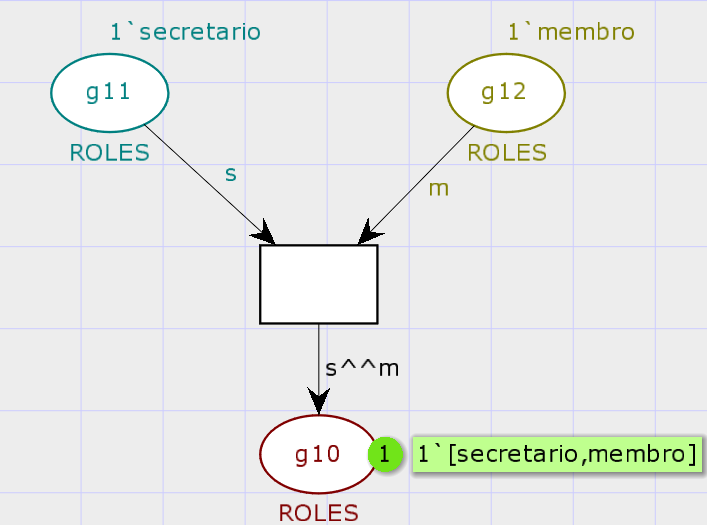
\includegraphics[width=0.45\textwidth]{imagens/4-rp-exemplo4.png}\label{fig:4-rp-exemolo4}}
  \caption{RPC metas $g11$, $g12$ e $g10$}
  \label{fig:RPC-2}
\end{figure}

Para completar a modelagem da RPC, deve-se incluir transições que serão ativadas quando uma meta falhar. É necessário incluir uma transição e um lugar de falha para cada lugar até então do modelo, uma transição auxiliar é necessária para realizar a ligação com o lugar final. Na Figura \ref{fig:4-rp-falha1} a simulação da RPC foi concluída pelo caminho esperado, já na Figura \ref{fig:4-rp-falha2} ocorreu uma falha. É possível observar que a inscrição do arco após a transição de falha possui uma função onde caso alguma das fichas entrar na transição a ficha resultante no lugar $g10$ será a de falha.

\begin{figure}[ht]
  \centering
  \subfigure[RPC com sucesso na execução ]{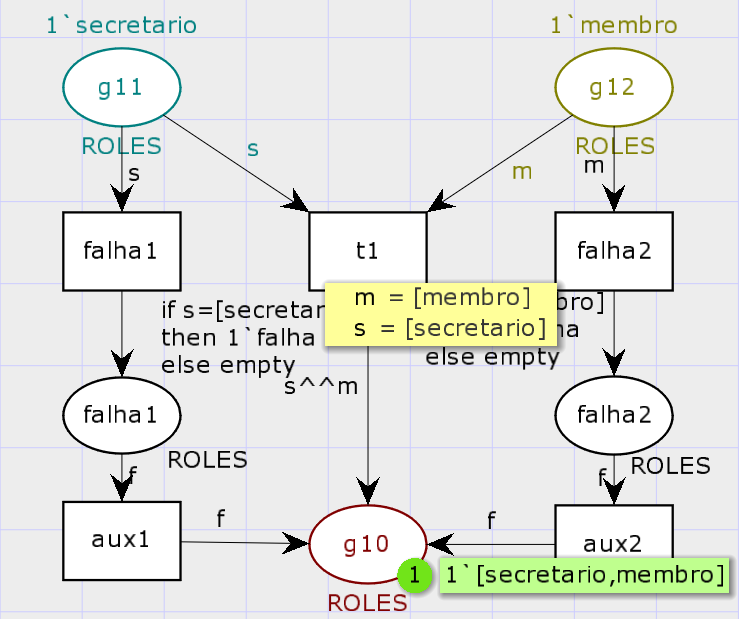
\includegraphics[width=0.49\textwidth]{imagens/4-exemploRPCOK.png}
  \label{fig:4-rp-falha1}}
  \subfigure[RPC com falha na execução]{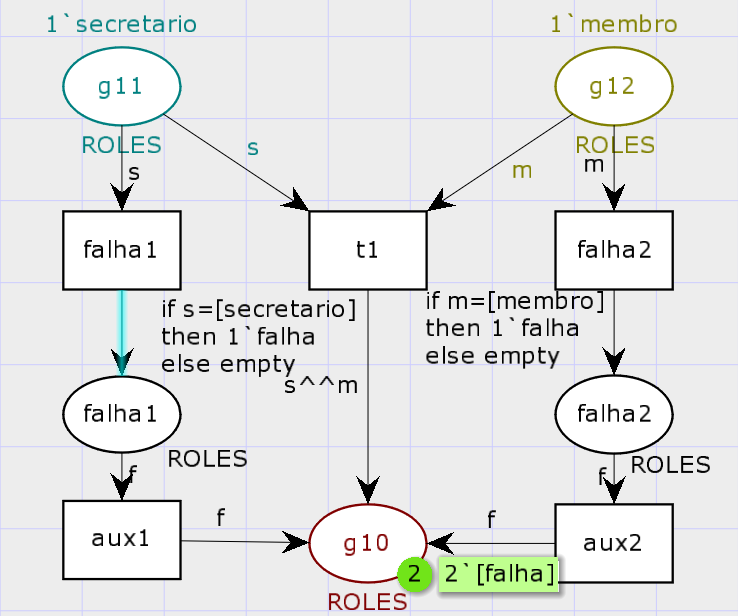
\includegraphics[width=0.49\textwidth]{imagens/4-exemploRPCFalha.png}\label{fig:4-rp-falha2}}
  \caption{RPC com uma transição de falha}
  \label{fig:RPC-3}
\end{figure}

A última etapa do processo é a contagem dos caminhos da RPC modelada. O programa CPN Tools não possui uma ferramenta para esta avaliação, para obter este resultado é utilizado um algoritmo de contagem de caminhos para grafos dirigidos. Para executar o algoritmo na rede é preciso a conversão em um grafo dirigido. 

Foi desenvolvida uma ferramenta Web\footnote[1]{disponível em https://github.com/brunocoelhor/PetriNet2Graph} para a conversão do arquivo do CPN Tool, a RPC, para um grafo dirigido. A ferramenta consiste no carregamento do arquivo com extensão $.cpn$, então este é convertido em um objeto \textit{JSON} para facilitar a obtenção das informações necessárias pelo Javascript.

Através da leitura do arquivo \textit{JSON} são convertidos os lugares, transições e arcos da RPC para os nós e arcos do grafo. Com estes dados é possível gerar um grafo e apresentar em tela através do biblioteca Cytoscape.js\footnote[2]{disponível em http://js.cytoscape.org/}.

Com as mesmas informações utilizadas para gerar o grafo em tela é gerado um \textit{array} nó-origem, nó destino que permite o algoritmo realizar a contagem dos caminhos. Logo o resultado da ferramenta é apresentado, as informações são: o número de lugares, transições, arcos e o total de caminhos e a estrutura do grafo gerado na transformação, o resultado pode ser visto na Figura \ref{fig:4-resultado}.

\begin{figure}[ht]
\centering
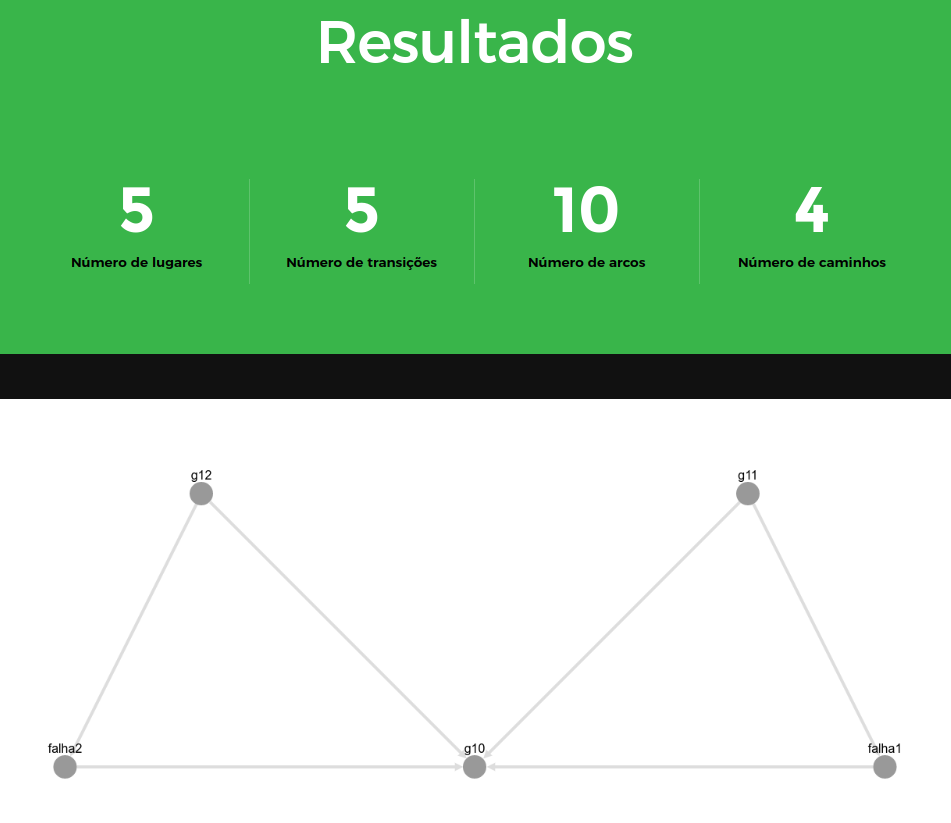
\includegraphics[scale=0.3]{imagens/4-resultado.png}
\caption{Resultados da RP.}
\label{fig:4-resultado}
\end{figure}


A Figura \ref{fig:4-fluxograma} representa o fluxograma das etapas do processo para a avaliação da testabilidade de um SMA utilizando $\mathcal{M}$oise$^{+}$ através da contagem de caminhos da RPC modelada do sistema.


\begin{figure}[ht]
\centering
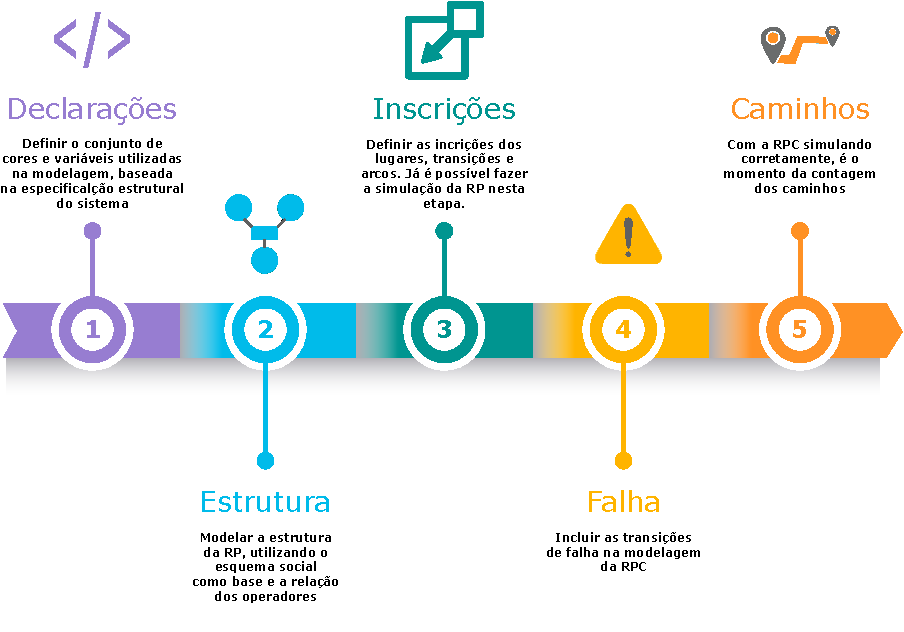
\includegraphics[scale=0.9]{imagens/4-fluxograma.pdf}
\caption{Etapas do processo.}
\label{fig:4-fluxograma}
\end{figure}

No capítulo seguinte a metodologia é implementada em dois estudos de caso. 